\chapter{Operational Amplifier}

\section{Tujuan Pembelajaran}

Setelah mempelajari bab ini, kalian diharapkan mampu untuk

\begin{enumerate}
	\item Menjelaskan karakteristik dari op amp ideal dan op amp 741.
	\item Menentukan \textit{slew rate} dan menggunakannya untuk mencari \textit{power bandwidth} dari op amp.
	\item Menganalisis op amp inverting amplifier.
	\item Menganalisis op amp noninverting amplifier.
	\item Menjelaskan cara kerja summing amplifier dan voltage follower.
	\item Menjelaskan IC linear lainnya dan mendiskusikan bagaimana penggunaannya.
\end{enumerate}

\section{Pengantar Op Amp}

Gambar \ref{fig:16.01} menunjukkan diagram blok dari op amp. \textit{Input stage} dari op amp tersebut adalah diff amp, kemudian dilanjukan oleh lebih banyak \textit{stage gain}/ penguat, dan sebuah \textit{Class-B push-pull emitter follower}. Karena diff amp berfungsi sebagai \textit{first stage}, maka diff amp yang akan menentukan karakteristik \textit{input} dari op amp. Pada sebagian besar op amp memiliki \textit{output} berupa \textit{single-ended}. Dengan positif dan negatif \textit{supply}, \textit{single-ended output} didisain untuk memiliki nilai diam (\textit{quiescent value}) nol. Artinya, tegangan \textit{input} nol idealnya menghasilkan tegangan \textit{output} nol.

\begin{figure}
	\centering
	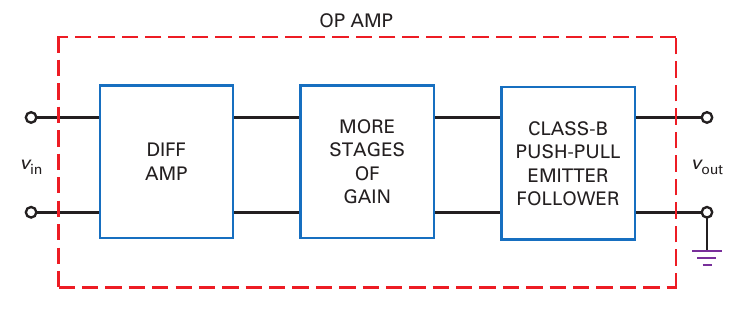
\includegraphics[width=0.7\linewidth]{pic/fig:16.01}
	\caption{Diagram blok dari op amp}
	\label{fig:16.01}
\end{figure}

Tidak semua op amp didesain seperti pada Gambar \ref{fig:16.01}. Misalkan, beberapa op amp tidak memiliki\textit{ Class-B push-pull output}, dan ada juga yang memiliki \textit{double-ended output}. Selain itu, op amp tidak sesederhana seperti yang ditunjukkan oleh Gambar \ref{fig:16.01}. Disain internal dari monolithic op amp sangatlah rumit, menggunakan ribuan transistor sebagai \textit{current mirror}, \textit{active load}, dan inovasi lainnya yang tidak mungkin ada di disain diskrit. Namun kita cukupkan sesuai dengan kebutuhan kita bahwa Gambar \ref{fig:16.01} menekankan pada dua fitur yang penting yaitu \textit{differential input} dan \textit{single-ended output}.

\begin{figure}
	\centering
	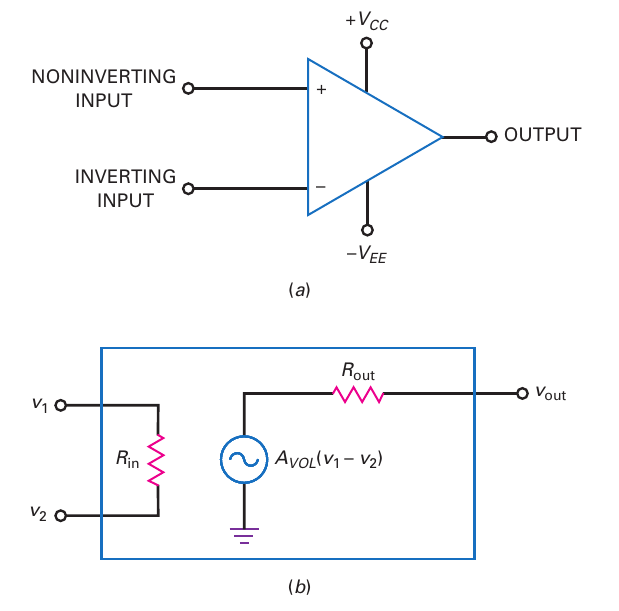
\includegraphics[width=0.7\linewidth]{pic/fig:16.02}
	\caption{(a) Simbol skematik dari op amp; (b) rangkaian ekivalen dari op amp}
	\label{fig:16.02}
\end{figure}

Gambar \ref{fig:16.02} adalah simbol skematik dari op amp. Pada gambar tersebut terdapat noninverting, inverting input dan single-ended output. Idealnya,